\documentclass[times,specification,annotation]{itmo-student-thesis}
\linespread{1.4}
%% Опции пакета:
%% - specification - если есть, генерируется задание, иначе не генерируется
%% - annotation - если есть, генерируется аннотация, иначе не генерируется
%% - times - делает все шрифтом Times New Roman, собирается с помощью xelatex
%% - languages={...} - устанавливает перечень используемых языков. По умолчанию это {english,russian}.
%%                     Последний из языков определяет текст основного документа.

%% Делает запятую в формулах более интеллектуальной, например:
%% $1,5x$ будет читаться как полтора икса, а не один запятая пять иксов.
%% Однако если написать $1, 5x$, то все будет как прежде.
\usepackage{icomma}

%% Один из пакетов, позволяющий делать таблицы на всю ширину текста.
\usepackage{tabularx}

%% Данные пакеты необязательны к использованию в бакалаврских/магистерских
%% Они нужны для иллюстративных целей
%% Начало
\usepackage{tikz}
\usetikzlibrary{arrows}
\usepackage{filecontents}
\begin{filecontents}{bachelor-thesis.bib}
@online{ big-graphs-future-arxiv,
    year        = {2020},
    title       = {The Future is Big Graphs! A Community View on Graph Processing Systems},
    author      = {Sherif Sakr and Angela Bonifati and Hannes Voigt and Alexandru Iosup and Khaled Ammar and Renzo Angles},
    url         = {https://arxiv.org/abs/2012.06171},
    year        = {2020},
    langid      = {english}
}

@online{ graph-db-scale,
    year        = {2022},
    title       = {Graph Database Scalability},
    author      = {Neo4j},
    url         = {https://neo4j.com/product/neo4j-graph-database/scalability/},
    year        = {2022},
    langid      = {english}
}

@online{ saner,
    year        = {2020},
    title       = {Ultra-Large-Scale Repository Analysis via Graph Compression},
    author      = {Paolo Boldi and Antoine Pietri and Sebastiano Vigna and Stefano Zacchiroli},
    url         = {https://upsilon.cc/~zack/research/publications/saner-2020-swh-graph.pdf},
    year        = {2020},
    langid      = {english}
}

@online{ scale-cost,
    year        = {2015},
    title       = {Scalability! But at what COST?},
    author      = {Frank McSherry and Michael Isard and Derek G. Murray},
    url         = {https://www.usenix.org/system/files/conference/hotos15/hotos15-paper-mcsherry.pdf},
    year        = {2015},
    langid      = {english}
}

@online{ gremlin,
    year        = {2022},
    title       = {Gremlin Query Language},
    author      = {{Apache TinkerPop}},
    url         = {https://tinkerpop.apache.org/gremlin.html},
    year        = {2022},
    langid      = {english}
}

@online{ swh-main-page,
    year        = {2022},
    title       = {Software Heritage},
    author      = {{Software Heritage}},
    url         = {https://www.softwareheritage.org/},
    year        = {2022},
    langid      = {english}
}

@online{ swh-intern,
    year        = {2022},
    title       = {TinkerPop Gremlin backend for WebGraph (internship)},
    author      = {{Software Heritage}},
    url         = {https://wiki.softwareheritage.org/wiki/TinkerPop_Gremlin_backend_for_WebGraph_(internship)},
    year        = {2022},
    langid      = {english}
}

@online{ webgraph,
    year        = {2022},
    title       = {WebGraph},
    author      = {WebGraph},
    url         = {https://webgraph.di.unimi.it/},
    year        = {2022},
    langid      = {english}
}

@online{ tinkerpop-enabled,
    year        = {2022},
    title       = {Data System Providers},
    author      = {{Apache TinkerPop}},
    url         = {https://tinkerpop.apache.org/providers.html},
    year        = {2022},
    langid      = {english}
}

@online{ tinkerpop,
    year        = {2022},
    title       = {Apache TinkerPop},
    author      = {{Apache TinkerPop}},
    url         = {https://tinkerpop.apache.org/},
    year        = {2022},
    langid      = {english}
}

@online{ git,
    year        = {2022},
    title       = {Git},
    author      = {{Git}},
    url         = {https://git-scm.com/},
    year        = {2022},
    langid      = {english}
}

@online{ swh-dataset,
    year        = {2022},
    title       = {Dataset - Software Heritage},
    author      = {{Software Heritage}},
    url         = {https://docs.softwareheritage.org/devel/swh-dataset/graph/dataset.html},
    year        = {2022},
    langid      = {english}
}


\end{filecontents}
%% Конец

%% Указываем файл с библиографией.
\addbibresource{bachelor-thesis.bib}

\begin{document}

\studygroup{M34391}
\title{Реализация TinkerPop инфраструктуры для WebGraph}
\author{Стародубцев Андрей Игоревич}{Стародубцев А.И.}
\supervisor{Аксенов Виталий Евгеньевич}{Аксенов В.Е.}{PhD, науки}{главный научный сотрудник Университета ИТМО}
\publishyear{2022}
%% Дата выдачи задания. Можно не указывать, тогда надо будет заполнить от руки.
\startdate{31}{января}{2022}
%% Срок сдачи студентом работы. Можно не указывать, тогда надо будет заполнить от руки.
\finishdate{15}{мая}{2022}
%% Дата защиты. Можно не указывать, тогда надо будет заполнить от руки.
\defencedate{9}{июня}{2022}

\addconsultant{Zacchiroli Stefano}{HDR, Full Professor}

\secretary{Штумпф С.А.}

%% Задание
%%% Техническое задание и исходные данные к работе
\technicalspec{Требуется реализовать инфраструктуру фреймворка для обработки графов Apache TinkerPop, позволяющую обрабатывать графы, сжатые фреймворком WebGraph. Это позволит обрабатывать графы очень больших размеров (десятки миллиардов вершин) при помощи экспрессивного доменно-ориентированного языка для обхода графов Gremlin. Для реализации требуется разработать программный слой, связывающий модели данных TinkerPop и WebGraph, реализовать структурные интерфейсы TinkerPop для WebGraph, добавить поддержку различных подходов к хранению свойств вершин/ребер, оценить производительность реализации на представляющих интерес запросах в конкретном домене (архив репозиториев Software Heritage), найти и исправить узкие места.}

%%% Содержание выпускной квалификационной работы (перечень подлежащих разработке вопросов)
\plannedcontents{TinkerPop - фреймворк изначально направленный на использование в графовых базах данных. При реализации для сжатых графов потребуется максимально оптимизировать слой, связывающий два фреймворка, чтобы не препятствовать масштабируемости.

Поскольку WebGraph не предоставляет единого способа хранения свойств вершин/ребер, необходимо разработать абстракции, которые позволят TinkerPop получать доступ и вычислять значения этих свойств во время исполнения запросов.

Для анализа производительности потребуется  реализовать на Gremlin ряд содержательных запросов в определенном домене, и замерить время их выполнения. Сравнение с нативными реализациями запросов позволит оценить практическую пользу реализации.}

%%% Исходные материалы и пособия
\plannedsources{\begin{enumerate}
    \item документация фреймворка для обработки графов Apache TinkerPop;
    \item документация фреймворка для сжатия графов WebGraph;
    \item документация Software Heritage.
\end{enumerate}}


%% ------ Конец части из ИСУ

%%% Цель исследования
\researchaim{Добавление возможности исполнения Gremlin запросов на графах, сжатых фреймворком WebGraph.}

%%% Задачи, решаемые в ВКР
\researchtargets{\begin{enumerate}
    \item реализация интерфейсов TinkerPop, позволяющих исполнять Gremlin запросы на графах, сжатых с использованием WebGraph;
    \item создание универсального механизма доступа к хранимым свойствам вершин и ребер, позволяющего использовать Gremlin запросы, опирающиеся на наличие/значения свойств;
    \item проведение анализа производительности реализации и сравнение с нативными реализациями запросов;
\end{enumerate}}

%%% Использование современных пакетов компьютерных программ и технологий
\addadvancedsoftware{Фреймворк \texttt{Apache TinkerPop}}{Список использованных источников}

%%% Краткая характеристика полученных результатов
\researchsummary{Разработана библиотека, позволяющая осуществлять немодифицирующие Gremlin запросы к любым графам, сжатым фреймворком WebGraph. Библиотека включает в себя поддержку различных источников свойств/вершин ребер, а также возможность определять собственные механизмы доступа к свойствам. Сформулирован ряд запросов в домене архивации данных систем контроля версий репозиториев с открытым исходным кодом, и проведен анализ производительности библиотеки на этих запросах.}

%%% Гранты, полученные при выполнении работы
\researchfunding{}

%%% Наличие публикаций и выступлений на конференциях по теме выпускной работы
\researchpublications{}

%% Эта команда генерирует титульный лист и аннотацию.
\maketitle{Бакалавр}

%% Оглавление
\tableofcontents

%% Макрос для введения. Совместим со старым стилевиком.
\startprefacepage

Графовое представление данных встречается все чаще \cite{big-graphs-future-arxiv}, а увеличение размеров таких графов приводит к необходимости использовать системы, которые справляются с масштабируемостью. Для графов малых/средних размеров могут использоваться графовые базы данных, предоставляющие достаточную производительность, а также широкие возможности для анализа данных с помощью запросов, сформулированных на специальных доменно-ориентированных языках, таких как Gremlin \cite{gremlin}. В случае больших графов (десятки миллиардов вершин, сотни миллиардов ребер) решением является сжатие графов. Фреймворк WebGraph \cite{webgraph} является единственным подобным решением и позволяет добиться хорошей производительности, в свою очередь, в отличие от графовых баз данных, требуя заметно меньше ресурсов \cite{graph-db-scale, scale-cost, saner}. Однако в данный момент такой подход предоставляет мало возможностей для анализа данных, поскольку способы доступы к вершинам и ребрам сжатого графа весьма лимитированы, и реализация запросов осуществляется вручную на каждый запрос, так как поддержки доменно-ориентированных языков для запросов WebGraph не предоставляют. Именно с такой проблемой столкнулась команда Software Heritage \cite{swh-main-page, swh-intern}, использующая фреймворк WebGraph для сжатия графа репозиториев \cite{saner}.

Целью данной работы является добавление поддержки Gremlin запросов для графов, сжатых фреймворком WebGraph. Это даст возможность осуществлять гибкие запросы к сжатым графам, что позволит удобным образом анализировать графы больших размеров, в частности граф репозиториев Software Heritage.

Первая глава содержит описание предметной области, а также постановку задачи. Во второй главе рассматриваются шаги, необходимые для достижения поставленной цели, а также описан подход к верификации решения. В третьей главе подробно описываются детали реализации основной части решения. Четвертая глава показывает, каким образом был проведен анализ производительности решения, и какие результаты были выявлены.

%% Начало содержательной части.
\chapter{Извлечение информации из графовых структур данных}

Многие задачи предполагают хранение данных в графовом представлении. Если пользователю необходимо извлечь некую информацию из этих данных, ему потребуется определить и выполнить некий запрос для этой структуры данных. Запрос может быть реализован нативно, то есть с использованием непосредственно методов низлежащей структуры. Такой подход не является гибким, так как требует ручной реализации на каждый отдельный случай. Альтернативой являются доменно-ориентированные языки для обхода графов, позволяющие формулировать гибкие запросы. Примером такого языка является язык Gremlin.

\section{Язык для обхода графов Gremlin}

Gremlin - доменно-ориентированный язык для обхода графов, разработанный компанией Apache \cite{gremlin}. Является самым популярным языком подобного рода с открытым исходным кодом, о чем свидетельствует его широкая поддержка множеством графовых баз данных \cite{tinkerpop-enabled}. Действительно, основной областью использования Gremlin являются графовые базы данных, и это становится заметно при рассмотрении возможностей Gremlin. Несмотря на это, Gremlin позволяет гибко формулировать любые запросы для любых графов, вне зависимости от самих данных.

\begin{lstlisting}[float=!h,caption={Пример запроса на Gremlin},label={lst1}]
g.V().has('code','LED')
     .repeat(out().simplePath())
     .until(has('code','SVO'))
     .path().by('code').limit(10)
\end{lstlisting}

 В Gremlin запросах пользователь может опираться как на структуру графа, то есть сами вершины и ребра, так и на свойства вершин и ребер. Свойства это дополнительная информация, хранящаяся в вершинах и ребрах. Примером такой информации может быть название аэропорта для графа рейсов, а примером свойства ребра может являться расстояние между аэропортами. 

Для исполнения запросов Gremlin использует библиотеку Apache TinkerPop \cite{tinkerpop}. Любая система имеет возможность реализовать инфраструктуру Apache TinkerPop (англ. TinkerPop-enabled system), что позволит исполнять в ней Gremlin запросы. Примерами подобных систем являются описанные ранее графовые базы данных.

\section{Ограничения графовых баз данных}

Предоставляя стандартную поддержку Gremlin, графовые базы данных дают возможность исполнять Gremlin запросы в своей системе - требуется лишь адаптировать свою систему под одну из таких баз данных. Такое решение хорошо подходит для графов малых/средних размеров. Однако, когда речь идет о больших графах (десятки миллиардов вершин, сотни миллиардов ребер), требуется масштабируемое решение. Графовые базы данных масштабируются за счет распределенных систем \cite{graph-db-scale}, на создание и поддержание которых требуются большие ресурсы.

\section{Сжатие графов}

Другим подходом к обеспечению хорошей производительности при работе с большими графами является сжатие графов. Такой подход позволяет существенно сократить размер графа в памяти. Это в свою очередь дает возможность разместить весь граф в оперативной памяти одного компьютера \cite{saner}, что существенно повышает эффективность доступа к графу, и позволяет анализировать его без использования распределенной системы. Стоит отметить, что под сжатием графа понимается сжатие именно его структуры, а не свойств. Единственным решением подобного рода с открытым исходным кодом является фреймворк WebGraph \cite{webgraph}.

\section{Ограничения WebGraph}

WebGraph позволяет эффективно хранить граф за счет сжатия его структуры, однако WebGraph не представляет поддержки Gremlin. Таким образом любой запрос к подобному графу требует реализации вручную, а WebGraph предоставляет весьма ограниченные способы доступа к структуре графа.
Помимо этого, WebGraph не предоставляет универсального способа для работы со свойствами вершин и ребер, работа с ними во многом становится обязанностью пользователя. При этом многие представляющие интерес запросы зависят от значений свойств вершин и ребер.

\section{Software Heritage}

Software Heritage - компания, занимающаяся архивированием данных систем контроля версий репозиториев с открытым исходным кодом. Архив представляет собой единый граф. Графовое представление обусловлено древовидным устройством распределенных систем контроля версий, таких как git \cite{git}. Структура графа приведена на рисунке~\ref{fig1}.

\begin{figure}[!h]
\caption{Структура архива Software Heritage}\label{fig1}
\centering
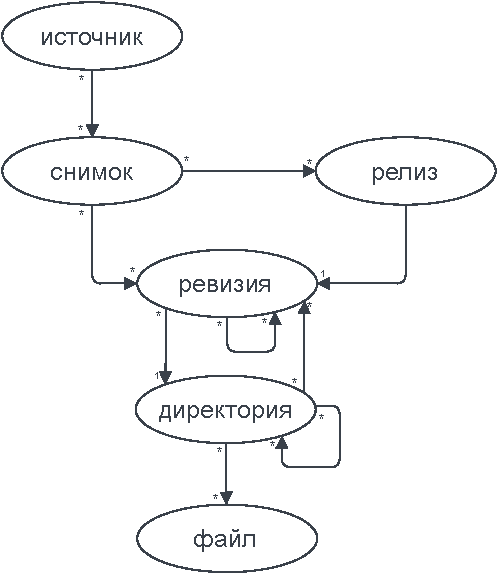
\includegraphics{swh-graph-structure.pdf}
\end{figure}

Единый граф архива содержит более двадцати миллиардов вершин и более двухсот тридцати миллиардов ребер \cite{swh-dataset}. При таком крупном размере графа, эффективное исполнение запросов на нем возможно при сжатии структуры графа, что позволяет разместить весь граф в менее чем ста гигабайтах оперативной памяти \cite{saner}. При этом для сжатия структуры используется описанный ранее фреймворк WebGraph.

Архив Software Heritage содержит больше количество информации, анализ которой может представлять интерес. Веб-сервер Software Heritage предоставляет доступ к набору 

\section{Постановка задачи}

Целью работы является реализация TinkerPop инфраструктуры для фреймворка для сжатия графов WebGraph. Это позволит выполнять сложные запросы на больших графах, используя язык Gremlin. Кроме того, необходимо добавить возможность указывать сторонние источники свойств вершин/ребер. После этого требуется сформулировать ряд запросов, анализ производительности исполнения которых покажет, насколько данный подход применим.

При этом, поскольку ключевое преимущество использования WebGraph перед графовыми базами данных, это возможность работать с большими графами на относительно слабой машине, реализация TinkerPop для WebGraph должна сохранить это преимущество. Поскольку TinkerPop предоставляет широкие возможности для обхода графов и в основном направлен на работу с графовыми базами данных, а WebGraph в свою очередь предоставляет весьма лимитированный API, фокусируясь на оптимизации памяти, потребуется максимально оптимизировать слой, связывающий эти два фреймворка.

\chapter{Подход к решению}

\section{Разбиение на подзадачи}

Для того, чтобы добиться поставленной задачи, потребуется:

\begin{enumerate}
    \item Реализовать интерфейсы Apache TinkerPop, превращающие WebGraph в TinkerPop-enabled систему
    \item Реализовать возможность указывать источники и способы доступа к свойствам вершин/ребер, для использования этих свойств в запросах
    \item Провести анализ производительности данной реализации
\end{enumerate}

\section{Реализация TinkerPop}

Для этого требуется реализовать для WebGraph интерфейсы пакета structure. Они включают в себя такие интерфейсы, как:
\begin{enumerate}
    \item Graph - основной интерфейс графа. Экземпляр позволяет получать доступ к вершинам и ребрам по идентификатору, либо ко всем сразу.
    \item Vertex - интерфейс вершины графа. Позволяет получить входящие/исхдящие вершины/ребра, а также доступные свойства
    \item Edge - интерфейс ребра графа. Позволяет получить входящие исходящие вершины, а также доступные свойства по уникальному ключу.
    \item Property - интерфейс свойства вершин/ребер. Предоставляет доступ к значениям свойств.
\end{enumerate}
Помимо описанных методов, TinkerPop поддерживает модифицирующие граф запросы. В данной работе эта возможность реализоваываться не будет. Также TinkerPop поддерживает мета-свойства для вершин - свойства вершин становятся элементами графа наравне с вершинами и ребрами. Это возможность также реализовываться не будет.

Поскольку данная реализация нацелена на случай, в котором пользователь уже использует фреймворк WebGraph, а значит располагает представлением сжатого графа, и уже имеет возможность исполнять на нем нативные запросы, однако хочеть получить возможность исполнять запросы и на Gremlin, следует рассматривать реализацию как библиотеку, получающую в том или ином виде сжатый WebGraph граф, и предоставляющаую таким образом возможность исполнять на нем запросы на Gremlin, делегируя описанные выше методы низлежащему сжатому графу, с добавлением требуемой пред- и пост-обработки аргументов и результатов.

Как было описано выше TinkerPop предоставляет абстракции для вершин и ребер и работает с их экземплярами. WebGraph в свою очередь, предоставляет доступ к вершинам, ссылаясь на их уникальный числовой идентификатор. Располагая индексом вершины можно получить итератор индексов вершин-соседей. Это означает, что для реализации прослойки потребутеся создавать объекты-обертки. Здесь можно рассматривать два подхода:
\begin{enumerate}
    \item Сопоставить каждой вершине (ребру) единственный объект, который будет возвращаться при любом доступе к данной вершине.
    \item Возвращать временные копии объекты при доступе к данной вершине - два различных запроса к одной вершине могут вернуть различные объекты, но с одинаковыми свойствами.
\end{enumerate}

Первый вариант подразумаеват создание единого реестра объектов, для получения гарантии идентичности возвращаемых объектов при различных запросах. Учитывая цель сохранить преимущество в использованиии памяти, получаемое за счет сжатия графа, этот подход не является лучшим выбором, так как создает дополнительную нагрузку на память, которая при участиии в обходе достаточного числа вершин, станет существенной проблемой.
Второй подход в свою очередь удобен своей гибкостью. Оставляя возможность создавать новые объекты при каждом новом обращении к вершине, он не исключает возможности внесения оптимизаций, для уменьшения общего числа аллокаций новых объектов.

\section{Реализация доступа к свойствам}

Вершины и ребра в графе могу тобладать свйоствами (например название аэропорта). Так как многие (если не большинство) запросов представляют интерес именно в привязке к свойствам графа, а не исключительно по его топологии, Gremlin предоставляет возможность формулировать запросы, зависящие от свойств. Свойства устроены как пара ключ-значение, где ключом является строка, а значением объект. Gremlin позволяет как проверять наличие свойства с данным ключом у данной вершины/ребра, так и получать его значение, а также использовать это значение, например для фиьтрации. TinkerPop в свою очередь предоставляет интерфейс Property, который используется для получение доступа к свойствам даннйо вершины/реабра.

WebGraph - фреймворк, сжимающий графы с точки зрения их структуры. WebGraph предоставляет единсвтенный способ работы со свойствами - по индексу вершины можно получить как индексы его соседей, так и индексы соседей с 'метками'. Эти метки можно считать свойством ребра - для каждого ребра можно хранить единственный объект метку. В осталтном работа со свойствами перекладывается на пользователя, в частности свойства вершин, хранение нескольких свойств для ребер.
При этом существует ряд стандартных практик, использующихся для хранения и получения доступа к свойствам. Для вершин может использоваться сериализация массива примитивов, в котором индекс соответвсует индексу вершины, а значение по индексу - значению свойства для вершины. Для того, чтобы пользовтель имел возмодность удобным образом задавать спсооб доступа к свойствам вершин и ребер, следует реализовать ряд классов, позволяющих как использовать стандартные методы хранения свойста, так и пользовательсике способы хранения свойств.

\section{Анализ производительности реализации}

При связке этих двух фреймворков могут возникнуть проблемы с производительностью - требуется как сохранить малый отпечаток в памяти, достигаемый сжатием графа, так и снизить накладные расходы, которые появляются при адаптации WebGraph к TinkerPop.
Для анализа производительности следует выбрать конкретный набор данных, представленнных в виде графа. Следует определить ряд запросов, представляющих на нем интерес. Затем требуется реализовать данные запросы на языке Gremlin, и, используя сжатое WebGraph представление данного графа, исполнить данные запросы, после чего проанализировать результаты по ряду метрик, таких как: время выполнения, используемая память, число вершин/ребер, затронутых в процессе исполнения, число результатов.
В качестве такого набора данных будет использоваться архив Software Heritage - данные систем контроля версий репозиториев с открытым исходным кодом. Графовое представление обусловлено архивацией данных распределенных систем контроля версий данных проектов, базирующихся на дереве хешей (точнее сказать не дерево, а ориентированный ациклический граф). Он содержит информацию о более чем 1 милларде коммитов из более чем 80 миллионов репозиториев. Для непсредственного тестирования будет использоваться часть полного архива, а именно python3k, содержащий данные о 3 тысячах популярных репозиториев на языке python. Граф насчитывает 46 миллионов вершин и 1.2 миллиарда ребер.

\chapter{Реализация}

\section{Реализация TinkerPop}

\printmainbibliography

\end{document}
